\section{Технологический раздел}

\subsection{Выбор языка и библиотеки для разработки средства сбора данных}

В качестве средства реализации была выбрана библиотека Telebot, так как:

\begin{enumerate}
	\item[1.] Функционал приложения не предусматривает сложных операций, в силу чего низкая производительность ЯП Python не скажется на скорости отклика системы;
	\item[2.] ЯП Python позволит в короткий срок реализовать и отладить программный продукт;
	\item[3.] ЯП Python позволит быстро разворачивать приложение на разнообразных операционных системах, поддерживающих интерпретатор Python;
	\item[4.] Telebot предоставляет более тонкую настройку и контроль над запросами и ответами API Telegram.
\end{enumerate}

\subsection{Выбор СУБД}

Для организации хранения данных и моделей задействована реляционная СУБД PostgreSQL~\cite{postgres}. Данный выбор обусловлен наличием реляционных отношений в описанной системе, а также количеством полей у каждой сущности меньше 10, таким образом, данная СУБД может удовлетворить все потребности при реализации.

\subsection{Интерфейс средства сбора данных}

На рисунках \ref{img:teleg1}-\ref{img:teleg4} представлен интерфейс реализованного Telegram-бота.

\begin{figure}[H]
	\centering
	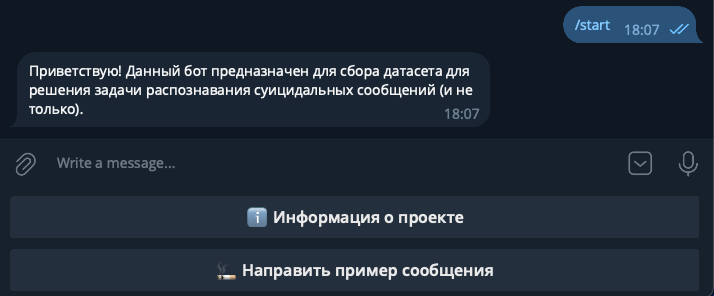
\includegraphics[width=\textwidth]{inc/teleg1.png}
	\caption{ Приветственное сообщение новому пользователю. }
	\label{img:teleg1}
\end{figure}

\begin{figure}[H]
	\centering
	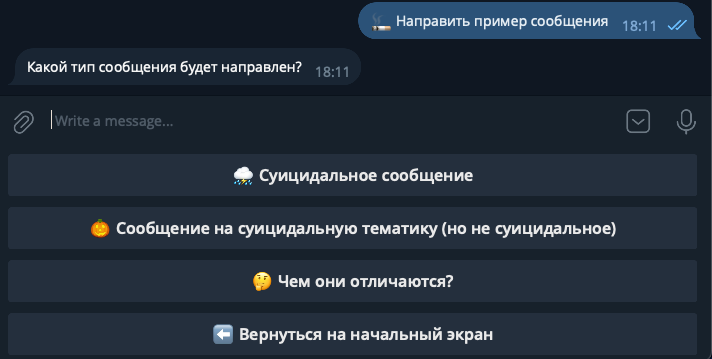
\includegraphics[width=\textwidth]{inc/teleg2.png}
	\caption{ Функционал направления в систему сообщения пользователем. }
	\label{img:teleg2}
\end{figure}

\begin{figure}[H]
	\centering
	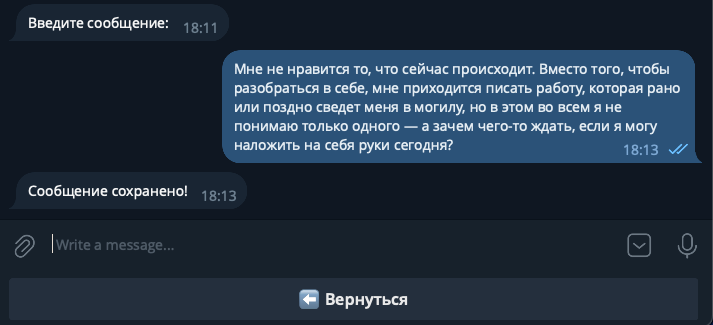
\includegraphics[width=\textwidth]{inc/teleg3.png}
	\caption{ Пример результата направленного в систему суицидального сообщения. }
	\label{img:teleg3}
\end{figure}

\begin{figure}[H]
	\centering
	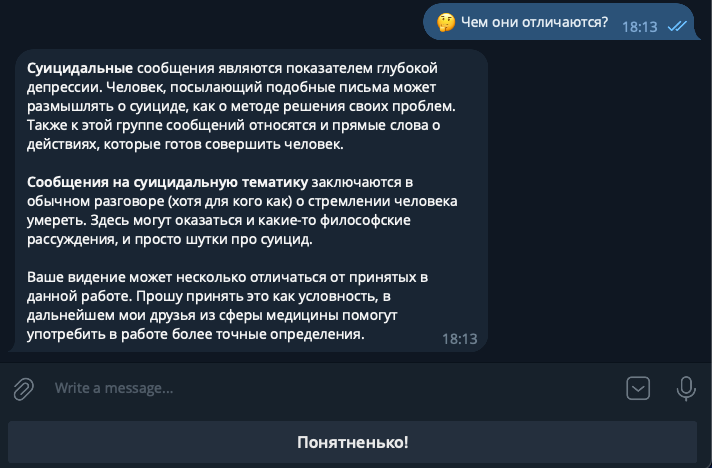
\includegraphics[width=\textwidth]{inc/teleg4.png}
	\caption{ Описание отличий суицидального сообщения и сообщения на суицидальную тематику. }
	\label{img:teleg4}
\end{figure}

\subsection{Описание обрабатываемых данных}

В результате работы средства сбора данных было размечено 1000 суицидальных сообщений. К собранным сообщениям было добавлено еще 1000 несуицидальных сообщений из датасета обнаружения пресуицидальных сигналов~\cite{dataset}. 

На рисунке \ref{img:cloud1} представлена визуализация собранных данных класса суицидальных сообщений. Из представленного облака слов видно, что чаще всего в суицидальных сообщениях фигурирует слова ``жизнь'', ``мочь'' и ``хотеть''. Также стоит обратить внимание на присутствие слов ``суицид'', ``страдать'', ``депрессия'', ``смерть'', ``умирать'' и ``ад''.

\begin{figure}[H]
	\centering
	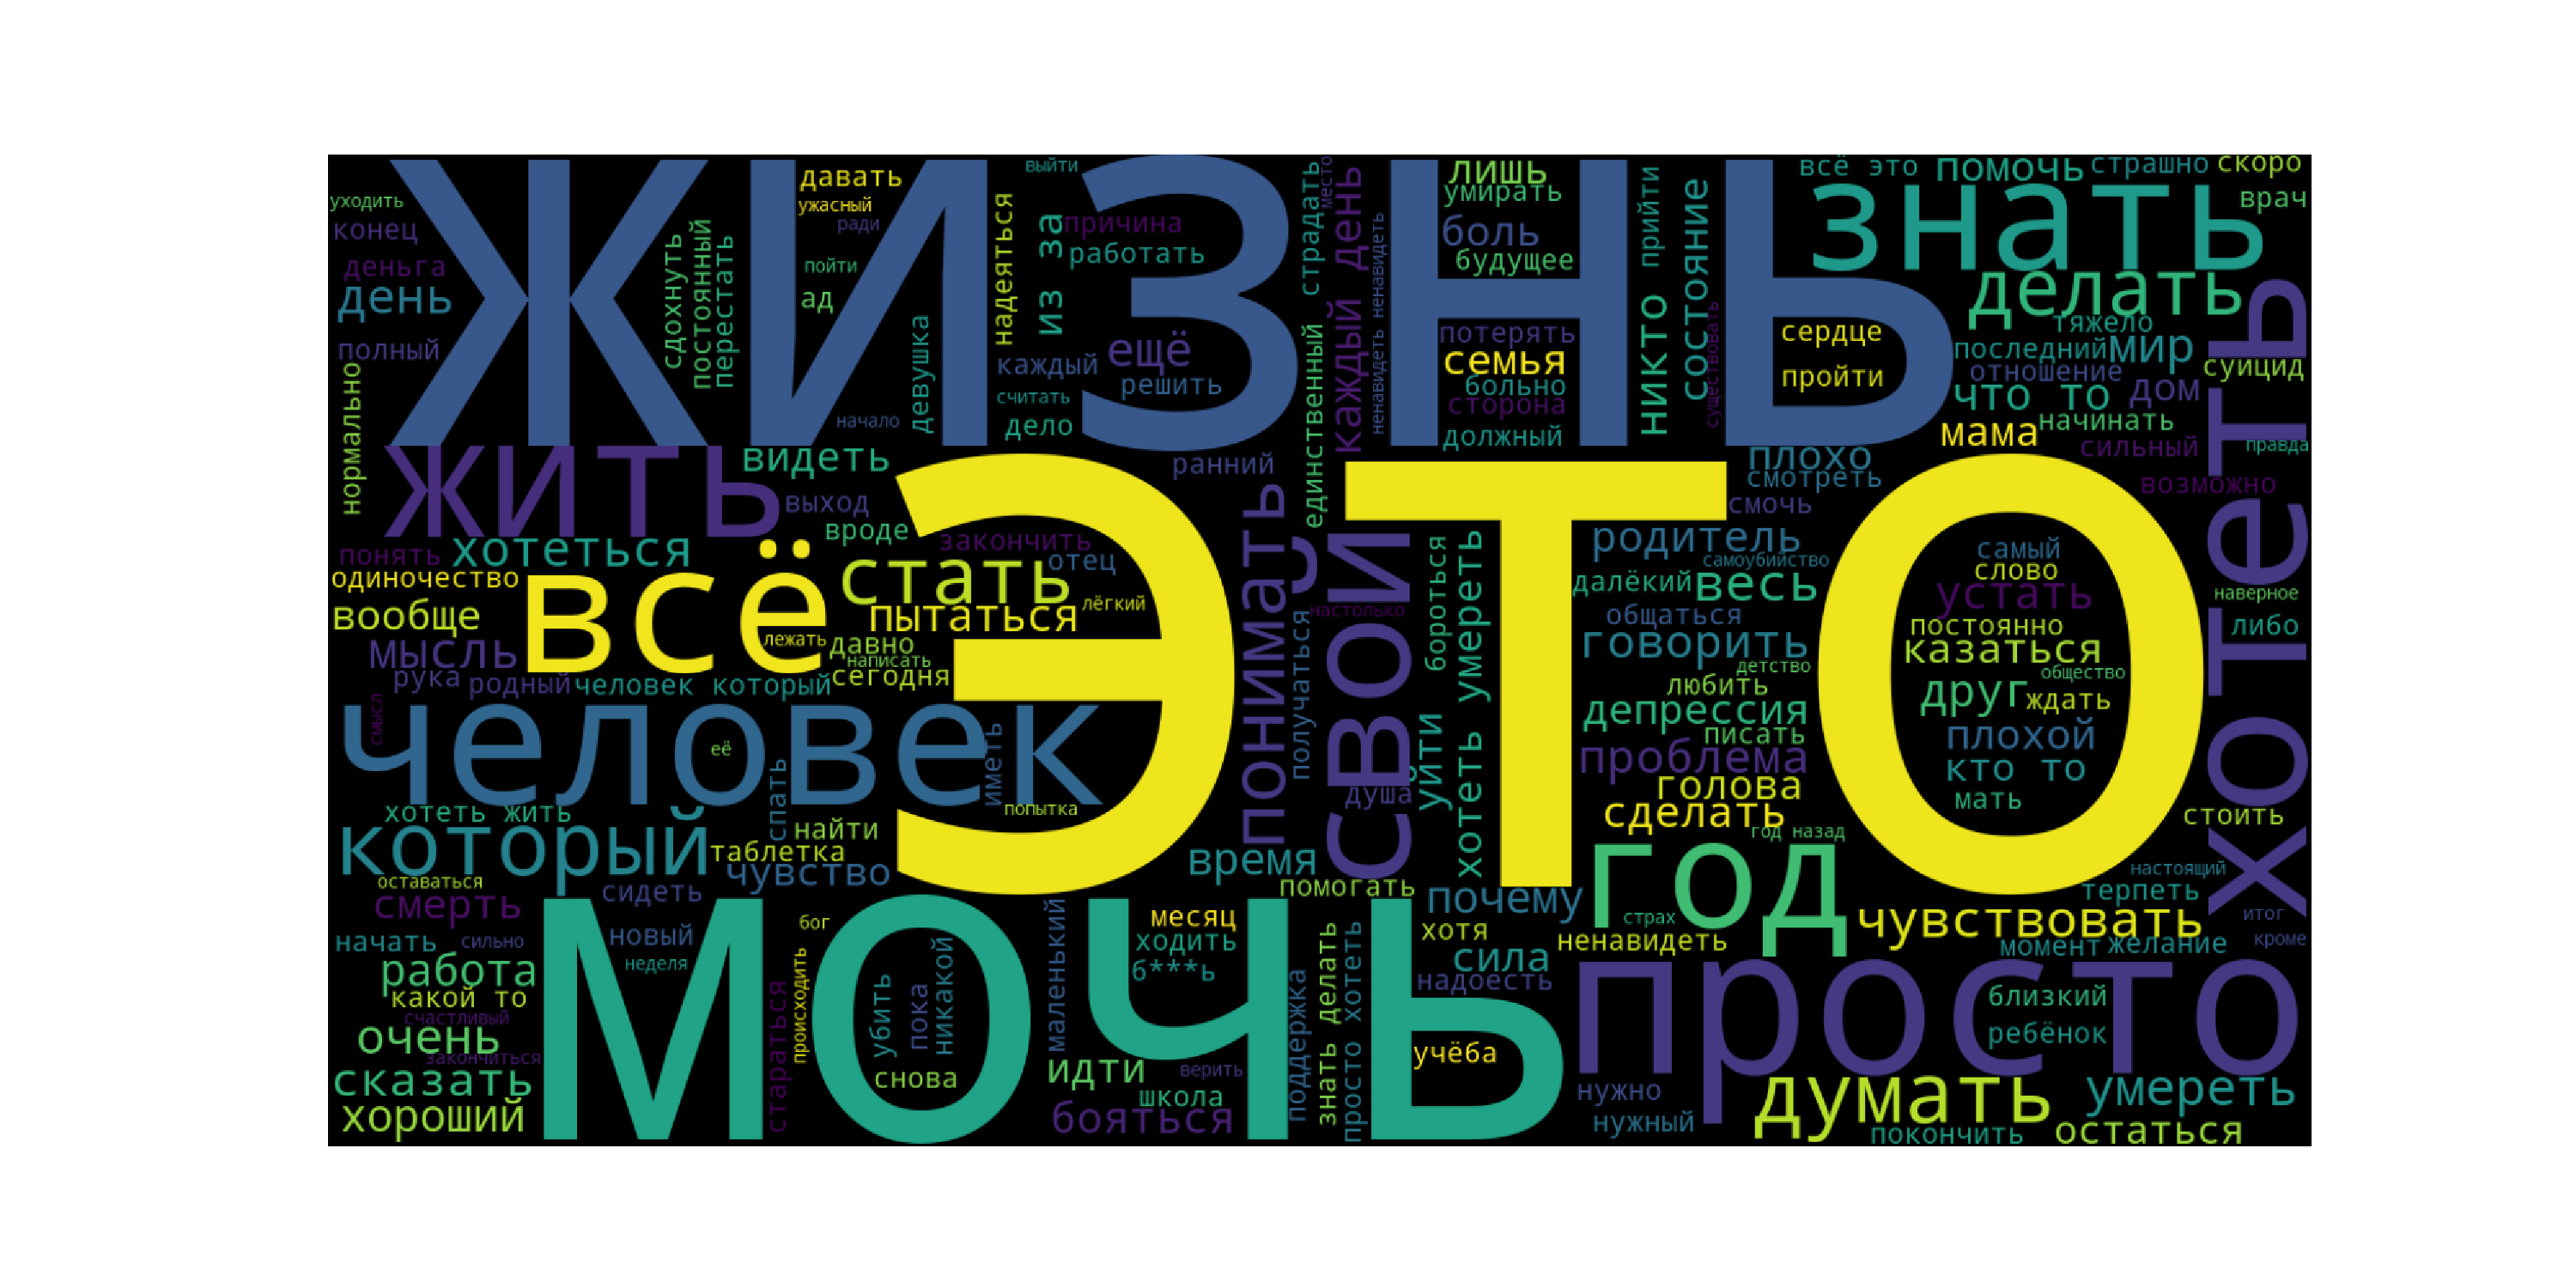
\includegraphics[width=\textwidth]{inc/cloudSuicidal.pdf}
	\caption{ Облако слов класса суицидальных сообщений. }
	\label{img:cloud1}
\end{figure}

На рисунке \ref{img:cloud2} представлена визуализация данных класса несуицидальных сообщений. Из представленного облака слов видно, что чаще всего в несуицидальных сообщениях встречаются слова ``хотеть'', ``человек'', а кроме того сообщения данной тематики чаще включают в себя различные вариации нецензурной брани.

\begin{figure}[H]
	\centering
	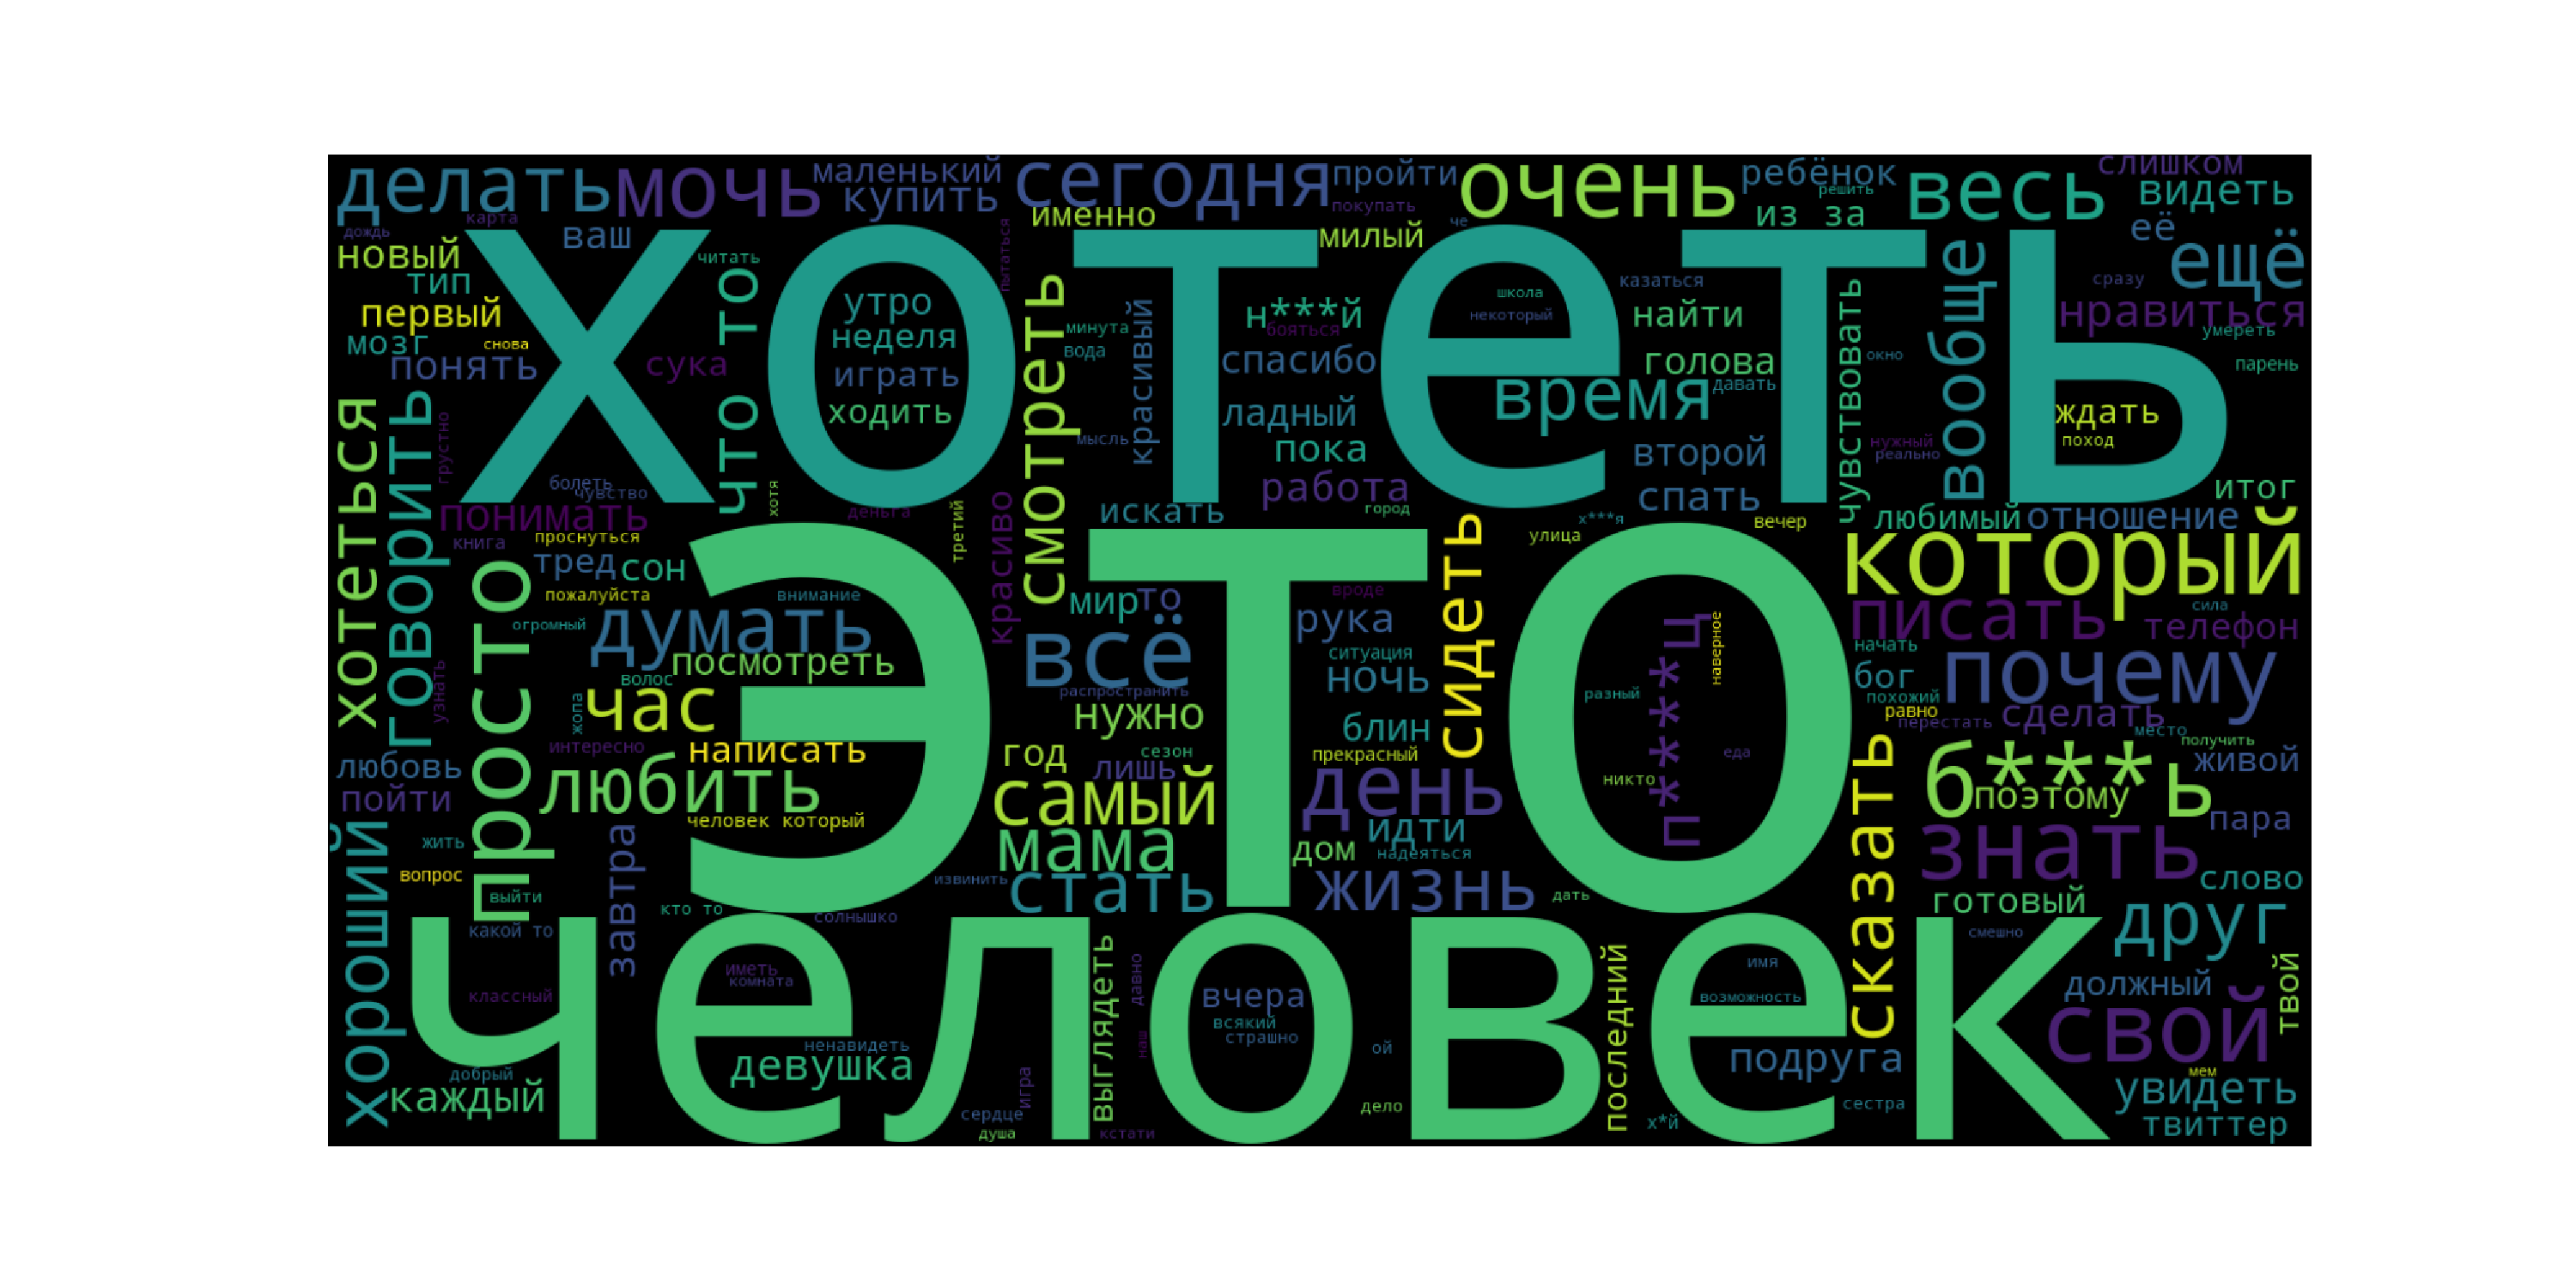
\includegraphics[width=\textwidth]{inc/cloudNonSuicidal.pdf}
	\caption{ Облако слов класса несуицидальных сообщений. }
	\label{img:cloud2}
\end{figure}

Представленная информация подтверждает факт того, что выбранные классы разделимы и отличны частотой употребления как слов, так и тематик.

\subsection{Выбор языка и библиотеки для разработки метода распознавания суицидальных паттернов поведения человека по текстовым сообщениям}

В качестве средства разработки метода распознавания суицидальных паттернов поведения человека по текстовым сообщениям использовался ЯП Python. Данный выбор обусловлен следующими факторами:

\begin{itemize}
	\item большое количество реализаций средств анализа и предобработки текста;
	\item широкий выбор библиотек для разработки в области машинного обучения;
	\item просто синтаксиса языка и высокая скорость разработки.
\end{itemize}

В качестве среды разработки был задействован Visual Studio Code. Данный выбор обусловлен тем, что это ПО распространяется по свободной лицензии, поставляется для конечного пользователя с открытым исходным кодом, а также имеет большое число расширений, ускоряющих процесс разработки.

Список задействованных библиотек:
\begin{itemize}
	\item padnas~\cite{pandas} -- библиотека для обработки и анализа данных;
	\item numpy~\cite{numpy} -- библиотека, добавляющая поддержку больших многомерных массивов и матриц, вместе с большой библиотекой высокоуровневых математических функций для операций с этими массивами;
	\item matplotlib~\cite{matplotlib} -- библиотека для визуализации данных;
	\item scikit-learn~\cite{sklearn} -- библиотека множества операций и алгоритмов, используемых в сфере науки о данных и машинном обучении;
	\item nltk~\cite{nltk} -- библиотека, предоставляющая обширный набор инструментов для работы с естественными языками;
	\item pymorphy2~\cite{pymorphy} -- библиотека, предоставляющая морфологический анализатор, а также утилиты для взаимодействия с ним.
\end{itemize}

\subsection{Интерфейс средства распознавания суицидальных паттернов поведения человека по текстовым сообщениям}

ОБСУЖДАЕМ С ЮРОЙ, АААААААААААААААААААААААА

Либо утилита для терминала с выбором модели, токенизатора и вводом сообщения, либо нативное приложение с тем же функционалом, либо API, разворачивающееся, но я в коко-джангу не хочу совсем... Либо делаем бота :))

\subsection*{Вывод}

wolol